\documentclass[a4paper,10pt]{article}
\usepackage[utf8]{inputenc}
\usepackage[margin=1.5cm, bottom=2cm]{geometry}
\usepackage{fancyhdr}
\usepackage{enumitem}
\usepackage{xcolor}
\usepackage[table]{xcolor}
\usepackage{makeidx}
\usepackage[most]{tcolorbox}
\newtcolorbox{osservazioni}{
  colback=gray!8,    % sfondo grigio chiaro
  colframe=white,      % nessun bordo
  arc=2mm,            % angoli smussati
  boxrule=0pt,        % spessore bordo 0
  fontupper=\footnotesize,
  left=2mm, right=2mm, top=2mm, bottom=2mm,
  before skip=7pt,   % niente spazio prima
  after skip=15pt     % niente spazio dopo
}
\newtcolorbox{osservazioni2}{
  colback=gray!8,    % sfondo grigio chiaro
  colframe=white,      % nessun bordo
  arc=2mm,            % angoli smussati
  boxrule=0pt,        % spessore bordo 0
  fontupper=\small,
  left=5mm, right=5mm, top=3mm, bottom=3mm,
  before skip=0pt,   % niente spazio prima
  after skip=30pt     % niente spazio dopo
}
\pagestyle{fancy}
\usepackage{tikz}
\usetikzlibrary{automata, positioning}
\pagestyle{fancy}

\usepackage{makeidx}

%%%%%%%%%%%%%%%%%%%
\newcommand{\EsercitazioneNum}{10}
\newcommand{\Data}{20/11/2025}
\newcommand{\DocType}{Esercitazione} % o "Eserciziario"
\newcommand{\FullTitle}{\DocType\ \EsercitazioneNum}

\newcommand{\Header}{
\noindent
  \small \textbf{Computabilità, Complessità e Logica - a.a. 2025/26} \hfill \textbf{\FullTitle} \\[0.2cm]
  \scriptsize Matteo Liotta, \texttt{matteo.liotta@studenti.units.it} \hfill \Data \\[0.2cm]
  \noindent\makebox[\linewidth]{\rule{\linewidth}{0.4pt}} \\[0.3cm]}

\newcommand{\NewPageHeader}{
  \vfill
  \noindent\makebox[\linewidth]{\rule{\linewidth}{0.4pt}}
  \newpage
  {\Header}
}
%%%%%%%%%%%%%%%%%%%

% Numero di pagina in basso al centro
\fancyhf{}
\fancyfoot[C] \thepage
\renewcommand{\footrulewidth}{0pt} % niente linea in basso
\renewcommand{\headrulewidth}{0pt} % niente linea in alto

\begin{document}

\footnotesize  % font generale più piccolo
\Header\\[0.7cm]


%%%%%%%%%%%%%%%% FOGLIO 2

    
    %% INDEX
    \addcontentsline{toc}{section}{Esercitazione 10: \textit{Logica Proposizionale}}
    
    \noindent\Large \textbf{Esercitazione 10}: \textit{Logica Proposizionale}
    \begin{osservazioni}
        \textbf{\textit{Nota}}. Sono indicati in \textcolor{blue}{\textit{blu}} gli esercizi che non saranno trattati durante l'esercitazione, bensì lasciati come strumento aggiuntivo di esercitazione individuale. Resta comunque assoluta disponibilità per la loro risoluzione negli incontri successivi, qualora necessario.
    \end{osservazioni}
    
    {\normalsize
    \begin{itemize}[label=, leftmargin=0pt]

    \item \textbf{\underline{Formule Booleane}}
    %% INDEX
    \addcontentsline{toc}{subsection}{Esercizio 1.} 
    %%
    \item \textbf{\textcolor{blue}{Esercizio 1.} (*)}\\ 	
    Si considerino le seguenti formule booleane:
    $$(A\rightarrow B)\lor(B\rightarrow A)$$
    $$(A \lor \lnot A)\rightarrow B$$
    $$(A \land \lnot A)\rightarrow B$$
    $$(A\rightarrow B)\land (B\rightarrow A)$$
    
    Si indichino, indicandone il motivo, quali sono delle \textit{tautologie}.
    

    %% INDEX
    \addcontentsline{toc}{subsection}{Esercizio 2.} 
    %%
    \item \textbf{\textcolor{blue}{Esercizio 2. }(*)}\\ 	
    Si considerino le seguenti formule booleane:
    $$(A\rightarrow B)\rightarrow C \quad e\quad (A\land \lnot B)\land\overline C$$
    $$(\lnot A \lor B\lor C)\land A \quad e \quad (B\lor C)$$
    Per ciascuna delle coppie indichi, giustificando il motivo, se la seconda è conseguenza logica della prima.
    
    %% INDEX
    \addcontentsline{toc}{subsection}{Esercizio 3.} 
    %%
    \item \textbf{Esercizio 3. (*)}\\ 	
    Data la seguente formula booleana:
    $$\phi:= (A\lor B) \rightarrow (B\lor C)$$
    
    Si indichino tutte le assegnazioni (o modelli) che verificano $\phi$, dunque si stabilisca se essa è \textit{soddisfacibile, una tautologia o insoddisfacibile}.\\[0.2cm]
    

    \item \textbf{\underline{Modellazione di problemi tramite formule booleane}}
    %% INDEX
    \addcontentsline{toc}{subsection}{Esercizio 4.} 
    %%
    \item \textbf{\textcolor{black}{Esercizio 4.} (*)}\\ 	
    Si scriva una formula booleana per modellare il seguente problema: dato un grafo della seguente forma,

    \begin{center}
    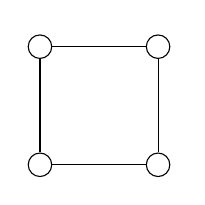
\begin{tikzpicture}[node distance=2cm, on grid, auto,
    state/.style={draw, circle, inner sep=3pt}]
        \node[state] (q0) {};
        \node[state, right=1.5of q0] (q1) {};
        \node[state, below=1.5of q0] (q2) {};
        \node[state, right=1.5of q2] (q3) {};
        
        \path
        (q0) edge node {} (q1)
        (q0) edge node {} (q2)
        (q1) edge node {} (q3)
        (q2) edge node {} (q3);
    \end{tikzpicture}
    \end{center}
    
    si indichi se possibile modellare la colorazione $\{0,1\}$ per ciascun nodo, in modo che \textit{vertici adiacenti non abbiano lo stesso colore}. 

    %% INDEX
    \addcontentsline{toc}{subsection}{Esercizio 5.} 
    %%
    \item \textbf{\textcolor{blue}{Esercizio 5.} (**)}\\ 
    Si consideri il del precedente esercizio: si scriva una formula booleana per modellare il problema della colorazione esteso al caso in cui ogni vertice è connesso a ciascun altro vertice, avendo a disposizione un totale di 3 colori.
    
    \begin{center}
    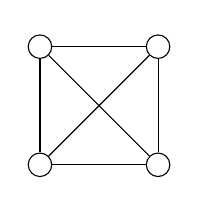
\begin{tikzpicture}[node distance=2cm, on grid, auto,
    state/.style={draw, circle, inner sep=3pt}]
        \node[state] (q0) {};
        \node[state, right=1.5of q0] (q1) {};
        \node[state, below=1.5of q0] (q2) {};
        \node[state, right=1.5of q2] (q3) {};
        
        \path
        (q0) edge node {} (q1)
        (q0) edge node {} (q2)
        (q1) edge node {} (q3)
        (q2) edge node {} (q3)
        (q0) edge node {} (q3)
        (q2) edge node {} (q1);
    \end{tikzpicture}
    \end{center}

    \NewPageHeader

    %% INDEX
    \addcontentsline{toc}{subsection}{Esercizio 6.} 
    %%
    \item \textbf{\textcolor{black}{Esercizio 6.} (***)}\\ 
    Si definisca una formula booleana per modellare un Sudoku 9x9. Si ricorda che:
    \begin{itemize}
        \item Ogni cella può contenere numeri da $1$ a $9$;
        \item Ogni cella deve essere tale che \textit{ogni riga contenga tutti i numeri da 1 a 9}, indipendentemente dall'ordine;
        \item Ogni sottogruppo 3x3 indicato in figura deve contenere tutti i numeri da 1 a 9.
    \end{itemize}


Si ricorda come lo schema del sudoku è il seguente:

\begin{figure}[h]
\begin{center}
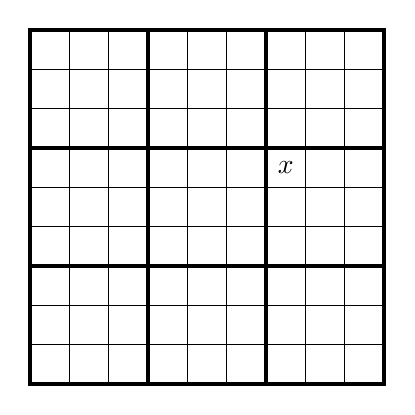
\begin{tikzpicture}[scale=0.5]
  % grid outer
  \draw[line width=1.2pt] (0,0) rectangle (9,9);

  % thin grid lines
  \foreach \i in {1,...,8}{
    \draw[line width=0.4pt] (\i,0) -- (\i,9);
    \draw[line width=0.4pt] (0,\i) -- (9,\i);
  }

  % thick 3x3 separators
  \foreach \k in {0,3,6,9}{
    \draw[line width=1.6pt] (\k,0) -- (\k,9);
    \draw[line width=1.6pt] (0,\k) -- (9,\k);
  }
  \node[] at (6.5,5.5) {$x$};

\end{tikzpicture}
\caption{Sudoku 9×9} 
\end{center}
\end{figure}


Dove si indichi $x = X_{r=4,c=7,k}\ , \quad k\in\{1,2,...,9\}$.
    

\end{itemize}

\vfill
\noindent\makebox[\linewidth]{\rule{\linewidth}{0.4pt}}
\end{document}